\documentclass[../Probability_Theory.tex]{subfiles}
\begin{document}
	\begin{center}
		\renewcommand{\arraystretch}{2}
		\begin{bfseries}
			\begin{tabular}{|c|}
				\hline
				Statistical Inference I \hfill Prof. Chin-Tsang Chiang\\
				\hspace{15em} {\large Lecture Notes 2} \hspace{15em}\ \\
				\lecdate \hfill Scribe: \scribe\\
				\hline
			\end{tabular}
			\renewcommand{\arraystretch}{1}
		\end{bfseries}
	\end{center}
On Monday, we define the idea of set and the operation over it. Intuitively, we think of the element of sets as an {\bf outcome} and think of a set as an {\bf event}. With these notion, further we want to design {\bf chance mechanism} on them to describe real world.

Here comes the important issues:
\begin{itemize}
	\item What kinds of domain (event space) for us to work on?
	\item What kind of chance mechanism (probability function) can we choose?
\end{itemize}
The critical concepts here is that we want to define {\bf axioms} for these two mathematical objects. Moreover, we want such axioms to be
\begin{itemize}
	\item Complete: Close under any possible operations.
	\item Compact: Less number of axioms as possible.
\end{itemize}

\section{Recall}
\subsection{limsup and liminf}
Intuitively, we think of sup and inf as:
\begin{itemize}
	\item sup: Upper bound. In set theory, we think of it as {\bf union} since it contains every future event.
	\item inf: Lower bound. In set theory, we think of it as {\bf intersection} since every future event contains it.
\end{itemize}
As a result, limsup and liminf is analogous to the {\bf asymptotic} upper bound and lower bound for a sequence of sets.

\subsection{Distributive law \& Partition}
\begin{enumerate}
	\item Consider events $A,B$ and sample space $\Omega$,
	$$B\cap\Omega=B\cap(A\cup A^C)=(B\cap A)\cup(B\cap A^C)$$
	As the sets in the union clause are a partition, distributive law tells us that we can divide the event $B$ into two parts. Here we consider a finite partition so you might not get the feeling. But imagine if the partition is infinite...?
	\item Consider,
	$$A\cup B=(A\cup B)\cap\Omega=(A\cup B)\cap(A\cup A^C)=A\cup(B\cap A^C)=A\cup (B\backslash A)$$
	Geometrically, it's like we union another set $B'=(B\backslash A)$ with $A$ where $A$ and $B'$ are {\bf disjoint}. In a special case: $A_1\supseteq A_2\supseteq ...$, it can be think of as a concentric circle
	\begin{figure}[h]
		\centering
		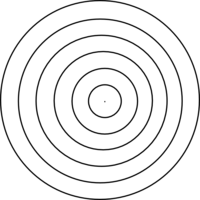
\includegraphics[scale=0.5]{concentric-circle.png}
	\end{figure}
	And thus we can transform an union into a {\bf disjoint union}.
\end{enumerate}

\subsection{General De Morgan's Law}
The De Morgan's law holds true as the number of sets is infinite! Formally, let $\{A_{\alpha}:\alpha\in\Gamma \}$, where $\Gamma$ is an index set and can be infinite, e.g. real line, or time segment. With such notation, we can define something like
$$\bigcup_{\alpha\leq t} A_{\alpha}$$
Which can be the events that happen before time $t$. Then, as De Morgan's law holds true, we can flip the union of events and consider the events that haven't show up. 

Intuitively we can think of this as the {\bf history} or {\bf filtration} in a {\it period sense}. And De Morgan's law provides a convenient way for us to do the computation.

\section{$\sigma$-Algebra}
\subsection{Intuitions and basic axioms}
By definition, $\sigma$-algebra is a collection of subsets of sample space. Intuitively, it is the space of meaningful events. As we mention the {\bf space} of events, $\sigma$-algebra must have some nice properties such as closeness under certain operations etc. But here what we concern is not only about what properties (axioms) a $\sigma$-algebra has to obey, but also about what's the most compact axioms we can have to capture the sufficient and necessary properties a $\sigma$-algebra should follow. And the answer is, there are three of axioms: Consider a $\sigma$-algebra $\mathcal{A}$ over sample space $\Omega$, 
\begin{enumerate}
	\item (contain empty event)$\emptyset\in\mathcal{A}$
	\item (close under complementation)$\forall A\in\mathcal{A}, A^C\in\mathcal{A}$
	\item (close under countable union)$\forall i\in\Gamma\ countable,\ A_i\in\mathcal{A},\ \bigcup_{i\in\Gamma}A_i\in\mathcal{A}$
\end{enumerate}
As a quick remark, we can see that with these axioms, we also have
\begin{itemize}
	\item $\Omega\in\mathcal{A}$ (by 1,2)
	\item Close under countable intersection (by 2, and De Morgan's law)
\end{itemize}

\subsection{Properties}
After defining the basic axioms for all $\sigma$-algebra, now a more applied issue arises:
$$What's\ the\ smallest\ \sigma-algebra?$$
With some observation, we can easily find out the largest and smallest $\sigma$-algebra over sample space $\Omega$ is
\begin{itemize}
	\item Trivial $\sigma$-algebra: $\{\emptyset,\Omega \}$
	\item Total $\sigma$-algebra: $\{A:A\subseteq\Omega \}$. That is, the power set of $\Omega$.
\end{itemize}
To answer this question, we have to clarify some concepts: How do we compare the size of two $\sigma$-algebras and to what extent do we want? The first question can be answered with strictly inclusion. If $\sigma$-algebra $\mathcal{A}_1$ strictly contains $\sigma$-algebra $\mathcal{A}_2$, then we can think of $\mathcal{A}_1$ is larger than $\mathcal{A}_2$. 

As to the second question, we can think this in a reverse way: What elements (subsets of $\Omega$) we must have? This question is problem-dependent, so here we imagine that we put all the events that we care into a set $A$. Then, we got a necessary condition for the $\sigma$-algebra that we desire: any $\sigma$-algebra that can describe the chance mechanism we're going to use must at least contain all the set in $A$.

Intuitively, with the above two concepts, it's reasonable to come to a wild guess for the minimal $\sigma$-algebra:
$$The\ intersection\ of\ all\ \sigma-algebras\ that\ contains\ A.$$
However, there's still one last thing to check: Is the (countable) intersection of $\sigma$-algebras also a $\sigma$-algebra? This can be proved in a theorem.
\begin{theorem}[$\sigma$-algebras are close under countable intersection]
	\mbox{}
	
	If $\mathcal{A}_{\alpha}$ is a $\sigma$-algebra $\forall \alpha\in\Gamma$, where $\Gamma$ is a countable index set. Then $\bigcap_{\alpha\in\Gamma}A_{\gamma}$ is also a $\sigma$-algebra.
\end{theorem}
\begin{proof}
	We should check three things and it's quite trivial. I believe I will never forget so here I leave it blank.
\end{proof}


\section{Probability Function}
Finally, it's time for us to construct the {\bf chance mechanism}! That is, we want to design probability function that maps from a $\sigma$-algebra to $[0,1]$. Moreover, such probability function should be analogous to real life. Namely, not every function from $\sigma$-algebra $\mathcal{A}$ to $[0,1]$ can be out candidate. As a result, we want to design rules (axioms) for probability function in advance. And just as the axioms for $\sigma$-algebra, we hope such axioms can be both compact and complete.

\paragraph{Komolgorov Axioms}
Consider sample space $\Omega$ and a $\sigma$-algebra $\mathcal{A}$ over it. Then, a probability function $P$ should satisfy the following axioms:
\begin{itemize}
	\item (Lower bound) $P(A)\geq0, \forall A\in\mathcal{A}$
	\item (Upper bound) $P(\Omega)=1$
	\item (Countably additive) If $A_{\alpha}\in\mathcal{A},\forall \alpha\in\Gamma$, where $\Gamma$ is a countable {\bf mutually exclusive} index set. Then, $P(\bigcup_{\alpha\in\Gamma}A_{\alpha})=\sum_{\alpha\in\Gamma}P(A_{\alpha})$
\end{itemize}
Note that this brings us from set functions to {\bf value function}. That is, we no longer playing only with set, but also take account the number, i.e. the probability.

Formally speaking, we say $(\Omega,\mathcal{A},P)$ is a probability space if $\mathcal{A}$ is a $\sigma$-algebra over $\Omega$ and $P$ is a probability function.

It's no hard to see that the most important axioms in Komolgorov axioms is countably additive. It allows us to deal with a countably infinite sequence of events. But you must wonder, can we relax the countably additive to finitely additive? If so, do we need to add other constraints? The answer is positive. In fact, we have
$$\mbox{Countably additive} = \mbox{Finitely additive} + \mbox{Axiom of continuity}$$

Here, we state the axiom of continuity without proof (left as exercise)
\begin{remark}
A measure is continuity from both below and above.
\end{remark}
\paragraph{Axiom of continuity}
If a sequence of events $A_1\supseteq A_2\supseteq...$ and $\lim_{n\rightarrow\infty}A_n=\emptyset$, then $\lim_{n\rightarrow\infty}P(A_n)=0$

After defining the axioms of probability function, now we want to design a probability function for our own usage. However, here comes the problem, how to assign probability function for a given usage? A simple theorem tells us that it's sufficient to define an unique probability function with the known probability assignments on {\bf trivial partition}.
\begin{theorem}
	Let sample space $\Omega=\{w_1,w_2,...\}$, assign probability value to each outcome as $p_1,p_2,...\geq0, \sum_i p_i=1$ respectively. Define the probability function $P$ as
	$$P(A):=\sum_{i:w_i\in A}p_i$$
\end{theorem}
With some verification to the axioms of probability function, we can see that $P$ is an unique probability function over $\Omega$ and the $\sigma$-algebra generated by partition $\{w_1,w_2,...\}$.

Intuitively, once we want to design a probability function for our chance mechanism, it's sufficient to assign probability values over a sufficient partition.

\begin{intuition}[Power set]
Someone must have questions about why we do not simply always pick power set to be our collection of events i.e. $\sigma$-algebra. This is because power set is so big that can contains non-measurable set which we can not define measure on it. Probability measure is just one kind of measure satisfying $\mu(\Omega)=1$. We must restrict our collection of events to those $\sigma$-algebra we are interested in and can define measure on. 
\end{intuition}
\section{Some random notes}

\subsection{Categorical classification/regression}
Suppose we are analyzing data with label set $\{A,B,C\}$ where these labels have no numerical meaning. What can we do? There's a simple solution called: {\bf dummy variable}

The idea is quite simple. Originally, we have a variable $s\in\{A,B,C\}$. But we cannot use $s$ in any regression or numerical model. Now, let's change a way of thinking. We no longer focus on {\bf which } label does $s$ take. Instead, we consider
\begin{align*}
&\mbox{Is $s$ takes label $A$?}\\
&\mbox{Is $s$ takes label $B$?}\\
&\mbox{Is $s$ takes label $C$?}
\end{align*}

Then, we generate {\bf two} dummy variables to {\bf quantify} the above intuition.
\begin{align*}
&x_1:=\left\{ \,
	\begin{IEEEeqnarraybox}[][c]{l?s}
	1,s=A\\
	0,else
	\end{IEEEeqnarraybox}
	\right.\\
&x_2:=\left\{ \,
\begin{IEEEeqnarraybox}[][c]{l?s}
1,s=B\\
0,else
\end{IEEEeqnarraybox}
\right.
\end{align*}

Now, we have two meaning dummy variables that can be fitted into a numerical model!

\subsection{Boole's inequality}
Boole's inequality, a.k.a union bound, provides a simple but useful tools when dealing with asymptotic issues.
\begin{theorem}[Boole's inequality]
	Consider set of events $\{A_{\alpha}:\alpha\in\Gamma\}$. Then we have
	$$P(\bigcup_{\alpha\in\Gamma}A_{\alpha})\leq\sum_{\alpha\in\Gamma}P(A_{\alpha})$$
\end{theorem}

From Boole's inequality, we can derive Borel Cantelli lemma. And from Borel Cantelli lemma, we can define the concept of almost surely convergence.


\end{document}




